\begin{multicols}{2}
    \section{Grundlagen}
    \subsection{Zahlen und Logik}
    \subsubsection{Zahlenbereiche}

    \begin{tabularx}{0.5\textwidth} {
            | >{\raggedright\arraybackslash}c
            | >{\raggedright\arraybackslash}X
            | >{\raggedright\arraybackslash}c |}
        \hline
        \textbf{*}     & \textbf{Bedeutung}                    & \textbf{Beispiel}                            \\ \hline
        $\mathbb{N}$   & Ganze Positive Zahlen                 & 1;2;3;                                       \\ \hline
        $\mathbb{N}_0$ & Ganze Positive Zahlen mit 0           & 0;1;2;                                       \\ \hline
        $\mathbb{Z}$   & Ganze Zahlen                          & -1;0;1;                                      \\ \hline
        $\mathbb{Q}$   & Rationale Zahlen = Bruchzahlen        & $\frac{3}{7} $ $\frac{5}{9} $ $\frac{2}{3} $ \\ \hline
                       & Irrationale Zahlen = Nachkommastellen & 0.3281                                       \\ \hline
        $\mathbb{R}$   & Reele Zahlen = Q + Irrationale Zahlen & Alle                                         \\ \hline
    \end{tabularx}

    \subsubsection{Summe und Produkte}
    \textbf{Summezeichen:} \\
    Es sei:  n, k $\in$ Z und n $\geq$ k
    \[ \sum_{k=1}^{n} a_k = a_1 + a_2 + a_3 + \ldots + a_n \]
    k heisst Laufvariable, Laufindex oder Summationsvariable \\
    1 heisst Startwert oder untere Grenze \\
    n heisst Endwert oder obere Grenze \\
    $a_{k}$ ist die Funktion bezueglich der Laufvariable \\

    \textbf{Produktzeichen:}
    \[ \prod_{k=1}^{n} a_k = a_1 \cdot a_2 \cdot a_3 \cdot \ldots \cdot a_n\]
    k heisst Laufvariable oder Laufindex \\
    1 heisst Startwert oder untere Grenze \\
    n heisst Endwert oder obere Grenze \\
    $a_{k}$ ist die Funktion bezueglich der Laufvariable \\

    \subsubsection{Mengen Operationen}

    \begin{tabularx}{0.5\textwidth} {
            | >{\raggedright\arraybackslash}c
            | >{\raggedright\arraybackslash}X |}
        \hline
        \textbf{*}            & \textbf{Bedeutung}                        \\ \hline
        $\varnothing$ oder {} & Leere Menge, enthaelt keine Elemente      \\ \hline
        $x\in A$              & Beschreibt Element x ist in Menge A       \\ \hline
        $x\notin A$           & Beschreibt Element x ist nicht in Menge A \\ \hline
        $A\subset B$          & A ist eine Teilmenge von B                \\ \hline
        $A\cap B$             & Schnittmenge von A und B                  \\ \hline
        $A\cup B$             & Vereinigunsgsmenge von A und B            \\ \hline
        $A\backslash B$       & Differenzbildung, Menge von A ohne B      \\\hline
    \end{tabularx}
    \\~\\
    \\~\\
    \\~\\

    \def\firstcircle{(0,0) circle (1cm)}
    \def\secondcircle{(0:1.2cm) circle (1cm)}

    \colorlet{circle edge}{blue!50}
    \colorlet{circle area}{blue!20}

    \tikzset{filled/.style={fill=circle area, draw=circle edge, thick},
        outline/.style={draw=circle edge, thick}}

    \setlength{\parskip}{5mm}
    % Set A and B
    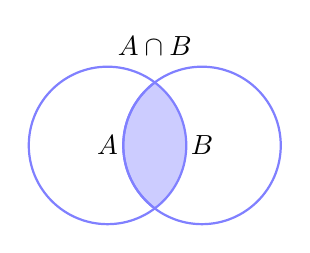
\begin{tikzpicture}
        \begin{scope}
            \clip \firstcircle;
            \fill[filled] \secondcircle;
        \end{scope}
        \draw[outline] \firstcircle node {$A$};
        \draw[outline] \secondcircle node {$B$};
        \node[anchor=south] at (current bounding box.north) {$A \cap B$};
    \end{tikzpicture}
    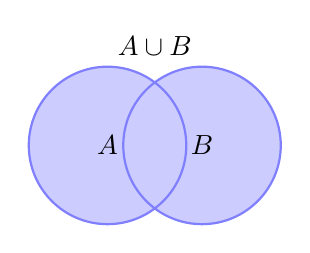
\begin{tikzpicture}
        \draw[filled] \firstcircle node {$A$}
        \secondcircle node {$B$};
        \node[anchor=south] at (current bounding box.north) {$A \cup B$};
    \end{tikzpicture}

    % Set A but not B
    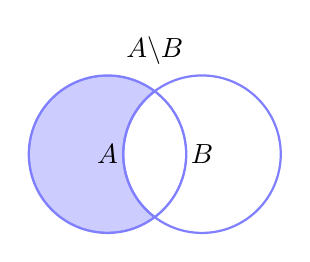
\begin{tikzpicture}
        \begin{scope}
            \clip \firstcircle;
            \draw[filled, even odd rule] \firstcircle node {$A$}
            \secondcircle;
        \end{scope}
        \draw[outline] \firstcircle
        \secondcircle node {$B$};
        \node[anchor=south] at (current bounding box.north) {$A\backslash  B$};
    \end{tikzpicture}
    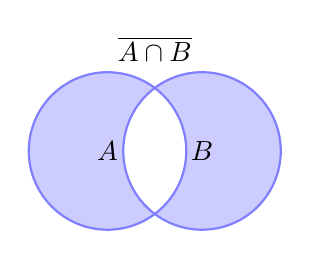
\begin{tikzpicture}
        \draw[filled, even odd rule] \firstcircle node {$A$}
        \secondcircle node{$B$};
        \node[anchor=south] at (current bounding box.north) {$\overline{A \cap B}$};
    \end{tikzpicture}


    \begin{tabularx}{0.5\textwidth} {
            | >{\raggedright\arraybackslash}c
            | >{\raggedright\arraybackslash}X
            | >{\raggedright\arraybackslash}c |}
        \hline
        \textbf{*}            & \textbf{Bedeutung}                         & \textbf{Beispiel}             \\ \hline
        $|A|$                 & Kardinalitaet/Maechtigkeit beschreibt      & A = {1;2}                     \\
                              & Anzahl Elemente einer Menge                & |$|A|$ = 2                    \\ \hline
        $\land$               & Konkuktion/UND A $\land$ B = Wahr wenn     & A $\land$ B                   \\
                              & A und B beide Wahr sind                    & A, B = W                      \\ \hline
        $\lor$                & Disjunktion/ODER A $\lor$ B  = Wahr wenn   & {-1;0;1;}                     \\
                              & A oder B  jeweils Wahr ist                 &                               \\ \hline
        $\neg$                & Negation A = Wahr$\neg$A = Falsch          & $\neg $A                      \\\hline
        $\implies$            & Implikation: Daraus folgt                  &                               \\ \hline
        $\Longleftrightarrow$ & aequivalenz A $\Longleftrightarrow$ B wenn &                               \\
                              & beide wahr oder falsch sind                &                               \\ \hline
        $\forall$             & Fuer Alle                                  & $\forall$ $x \in \mathbb{N}$  \\ \hline
        $\exists$             & Es Existiert                               & $\exists $ $x \in \mathbb{N}$ \\ \hline
    \end{tabularx}

    \begin{tabular}{@{ }c@{ }@{ }c | c@{ }@{ }c@{ }@{ }c@{ }@{ }c@{ }@{ }c | c@{ }@{ }c@{ }@{ }c@{ }@{ }c@{ }@{ }c | c@{ }@{ }c | c@{ }@{ }c@{ }@{ }c@{ }@{ }c@{ }@{ }c@{ }@{ }c}
        A & B &  & A & $\land$            & B &  &  & A & $\lor$             & B &  & $\lnot$            & B &  & A & $\lor$             & $\lnot$ & B & \\
        \hline
        T & T &  & T & \textcolor{red}{T} & T &  &  & T & \textcolor{red}{T} & T &  & \textcolor{red}{F} & T &  & T & \textcolor{red}{T} & F       & T & \\
        T & F &  & T & \textcolor{red}{F} & F &  &  & T & \textcolor{red}{T} & F &  & \textcolor{red}{T} & F &  & T & \textcolor{red}{T} & T       & F & \\
        F & T &  & F & \textcolor{red}{F} & T &  &  & F & \textcolor{red}{T} & T &  & \textcolor{red}{F} & T &  & F & \textcolor{red}{F} & F       & T & \\
        F & F &  & F & \textcolor{red}{F} & F &  &  & F & \textcolor{red}{F} & F &  & \textcolor{red}{T} & F &  & F & \textcolor{red}{T} & T       & F & \\
    \end{tabular}


    \subsection{Aussagenlogik}
    \vspace{-4mm}
    \subsubsection{Definitionen}
    \vspace{-4mm}
    \textbf{Term:}  Ein Term ist eine sinnvolle Zusammensetzung von Zahlen,
    Variablen, Operationszeichen und Klammern.
    Ein Term hat keinen Wahrheitsgehalt, ist also weder wahr noch falsch. \\
    \textbf{Aussage:}
    Eine Aussage beschreibt durch Worte oder Zeichen einen Sachverhalt.
    Eine Aussage ist entweder wahr oder falsch. \\
    \textbf{Aussageform:}
    Jeder sprachliche oder zeichensymbolische Ausdruck mit wenigstens einer Variablen
    wenn er durch jede sinnvolle Belegung der Variablen jeweils eine Aussage wird.

    \newpage

    \section{Gleichungen}
    \vspace{-4mm}
    \subsection{Allgemein}
    \vspace{-4mm}
    \subsubsection{Definitionen}
    \vspace{-4mm}
    \textbf{Gleichungen Loesen} \\
    Jede Zahl aus der Definitionsmenge, die beim Einsetzen fuer x zu einer wahren Aussage fuehrt, heisst Loesung der Gleichung. \\
    \textbf{Grundmenge, Definitionsbereich} $\mathbb{D}$ \\
    Die Menge aus der die Loesungen stammen duerfen. \\
    \textbf{Loesungsvariable} \\
    Variable nach der aufgeloest wird. \\
    \textbf{Formvariablen, Parameter} \\
    Alle anderen Variablen. \\
    \textbf{Loesungsmenge} \\
    Menge aller Elemente aus der Definitionsmenge, die zu einer wahren Aussage fuehren. \\
    \textbf{Aequivalenz} \\
    Zwei Gleichungen sind aequivalent, wenn beim Ersetzen der Variablen durch die gleichen Elemente der "gemeinsamen" Definitonsmenge entweder beide in eine wahre oder falsche Aussage uebergehen.

    \subsubsection{Aequivalenzumformungen}
    \vspace{-4mm}
    Umformungen einer Gleichung, bei denen die Loesungsmenge gleich bleibt, heissen aequivalenzumformungen.\\~\\
    \textbf{1. Termunformungen}\\
    $2x+5-3=0$ $\Longleftrightarrow$ $2x +2 = 0$ \\
    \textbf{2. Add./Sub.. mit der gleichen Zahl auf beiden Seiten} \\
    \textbf{3. Mult./Div. mit der gleichen Zahl auf beiden Seiten} \\
    Achtung: Ausser mit 0 \\
    \textbf{4. Beidseitige Add./Sub. mit dem gleichen Term} \\
    \textbf{5. Beidseitige Mult./Div. mit dem gleichen Term}

    \subsection{Lineare Gleichungen}
    \vspace{-4mm}
    \subsubsection{Definition}
    \vspace{-4mm}
    Eine Gleichung, die sich durch aequivalenzumformungen in die Form $ax + b = 0$ bringen laesst, heisst lineare Gleichung. Wir koennen lineare Gleichungen daran erkennen, dass die Variable nur in der 1. Potenz auftritt, also kein $x^2$, $x^3$\dots enthalten.

    \subsubsection{Loesen einer linearen Gleichung}
    \begin{enumerate}
        \item Gleichung nach $x$ aufloesen
        \item Loesungsmenge aufschreiben
    \end{enumerate}

    \subsection{Quadratische Gleichungen}
    \vspace{-4mm}
    \subsubsection{Definition}
    \vspace{-4mm}
    Gleichungen, die sich durch aequivalenzumformungen auf die Form $ax^2 + bx + c = 0 \quad (a, b, c \in \mathbb{R}; a \neq 0)$
    bringen lassen, heissen quadratische Gleichungen. Wir koennen quadratische Gleichungen daran erkennen, dass die Variable $x$ in der 2. Potenz $x^2$, aber in keiner hoeheren Potenz vorkommt. Es gibt 4 Arten/Formen von Quadratischen Gleichungen.
    \subsubsection{Loesen einer quadratischen Gleichung}
    \vspace{-4mm}
    \textbf{Loesung einer Reinquadratische Gleichung $ax^2 = 0$}
    Reinquadratische Gleichungen ohne Absolutglied besitzen als einzige Loesung die Null.

    \begin{enumerate}
        \item Gleichung nach $x^2$ aufloesen
        \item Wurzel ziehen
        \item Loesungsmenge aufschreiben
    \end{enumerate}
    \textbf{Beispiel Loesung einer Reinquadratische Gleichung mit Absolutglied $ax^2 + c = 0$}

    \begin{enumerate}
        \item Gleichung nach $x^2$ aufloesen
        \item Wurzel ziehen
        \item Loesungsmenge aufschreiben
    \end{enumerate}
    \textbf{Beispiel Loesung einer Gemischtquadratische Gleichungen ohne Absolutglied $ax^2 + bx = 0$}

    \begin{enumerate}
        \item Quadratische Gleichung in Normalform bringen
        \item $x$ ausklammern
        \item  Faktoren gleich Null setzen
        \item Gleichung nach $x^2$ aufloesen
        \item Loesungsmenge aufschreiben
    \end{enumerate}

    \subsubsection{Mitternachtsformel}
    \vspace{-4mm}
    Gemischtquadratische Gleichungen $ax^2 + bx + c = 0$ mit Absolutglied loesen wir mit der Mitternachtsformel:
    \[x_{1/2} = \frac{-b \pm \sqrt{b^2 - 4ac}}{2a}\]\\~\\
    Fallunterscheidung:
    \[x_{1} = \dfrac{-b - \sqrt{b^2 - 4ac}}{2a}\]
    \[x_{2} = \dfrac{-b + \sqrt{b^2 - 4ac}}{2a}\]\\~\\

    \textbf{Uebersicht}\\~\\
    \begin{tabularx}{0.5\textwidth} {
            | >{\raggedright\arraybackslash}X
            | >{\raggedright\arraybackslash}X
            | >{\raggedright\arraybackslash}X |}
        \hline
        \textbf{}                               & \textbf{Allgemeine Form}                       & \textbf{Normalform}                           \\ \hline
        Reinquadratisch ohne Absolutglied       & $2x^2 = 0$, $a = 2$, $b = 0$ und $c = 0$       & $x^2 = 0$, $a = 1$, $b = 0$ und $c = 0$       \\\hline
        Reinquadratisch mit Absolutglied        & $2x^2 -8 = 0$, $a = 2$, $b = 0$ und $c = -8$   & $x^2-4 = 0$, $a = 1$, $b = 0$ und $c = -4$    \\ \hline
        Gemischtquadrat- isch ohne Absolutglied & $2x^2-8x = 0$, $a = 2$, $b = -8$ und $c = 0$   & $x^2 -4x= 0$,  $a = 1$, $b = -4$ und $c = 0$  \\ \hline
        Gemischtquadrat- isch mit Absolutglied  & $2x^2-8x+6 = 0$, $a = 2$, $b = -8$ und $c = 6$ & $x^2-4x+3 = 0$, $a = 1$, $b = -4$ und $c = 3$ \\ \hline
    \end{tabularx}

    \textbf{Regeln}\\~\\
    Wenn das lineare Glied fehlt, gilt b = 0. \\
    Wenn das absolute Glied fehlt, gilt c = 0. \\
    Wenn das $x^2$ allein steht, gilt a = 0 (wegen $1 \cdot x^2 = x^2$).
    Wenn das x allein steht, gilt (wegen $1 \cdot x = x$).

    \textbf{Loesen einer Quadratischen Gleichung mit Mitternachtsformel}

    \begin{enumerate}
        \item Quadratische Gleichung in allgemeine Form bringen
        \item a, b und c aus der allgemeinen Form herauslesen
        \item  a, b und c in die Mitternachtsformel einsetzen
        \item Loesung berechnen
        \item Loesungsmenge aufschreiben
    \end{enumerate}

    \subsection{Bruchgleichung}
    \vspace{-4mm}
    \subsubsection{Definition}
    \vspace{-4mm}
    Eine Bruchgleichung ist eine Gleichung mit mindestens einem Bruchterm, in dem die Variable x im Nenner vorkommt.
    \subsubsection{Loesen einer Bruchgleichung}
    \vspace{-4mm}
    \begin{enumerate}
        \item Definitionsmenge bestimmen
        \item Gleichung nach $x$ aufloesen
        \item Pruefen, ob der x-Wert in der Definitionsmenge ist
        \item Loesungsmenge aufschreiben
    \end{enumerate}
    \subsubsection{Kehrwert}
    \vspace{-4mm}
    Wenn die Zaehler der Brueche nur aus Zahlen bestehen, kann eine Kehrwertbildung sinnvoll sein.
    Den Kehrwert eines Bruchs erhaelt man durch Vertauschen von Zaehler und Nenner.\\~\\
    \[\frac{{\colorbox{yellow}{$1$}}}{{\colorbox{orange}{$x$}}} = \frac{{\colorbox{yellow}{$2$}}}{{\colorbox{orange}{$x+1$}}} \Rightarrow  \frac{{\colorbox{orange}{$x$}}}{{\colorbox{yellow}{$1$}}} = \frac{{\colorbox{orange}{$x+1$}}}{{\colorbox{yellow}{$2$}}}\]


    \subsubsection{Multiplikation uebers Kreuz}
    \vspace{-4mm}
    Wenn auf beiden Seiten der Gleichung jeweils ein Bruch steht, kann eine Multiplikation ueber Kreuz sinnvoll sein.
    \[\frac{{\colorbox{yellow}{$1$}}}{{\colorbox{orange}{$x$}}} = \frac{{\colorbox{orange}{$2$}}}{{\colorbox{yellow}{$x+1$}}} \Rightarrow {\colorbox{yellow}{$1$}} \cdot {\colorbox{yellow}{$x+1$}} = {\colorbox{orange}{$2$}} \cdot {\colorbox{orange}{$x$}}\]


    \subsection{Betragsgleichung}
    \vspace{-4mm}
    \subsubsection{Definition}
    \vspace{-4mm}
    Betragsgleichungen lassen sich durch Fallunterscheidung loesen.

    \begin{equation*} |a| = \begin{cases} a &\text{fuer } a \geq 0 \\[5px] -a &\text{fuer } a < 0 \end{cases} \end{equation*}\\~\\
    Aus der Definition des Betrags ergeben sich folgende zwei Faelle: \\
    \begin{itemize}
        \item Wenn der Term im Betrag groesser oder gleich Null ist ($a \geq 0$), koennen wir den Term einfach ohne Betragsstriche schreiben ($|a| = a$)
        \item Wenn der Term im Betrag kleiner als Null ist ($a < 0$) , muessen wir die Vorzeichen des Terms umdrehen, um die Betragsstriche weglassen zu koennen ($|a| = -a$).
    \end{itemize}
    Die Loesungsmengen der einzelnen Faelle geben wir als Intervalle an. \\
    Die Loesungmenge der Gleichung ist die Vereinigungsmenge der einzelnen Loesungsmengen.\\~\\
    \textbf{Fallunterscheidung}
    \begin{enumerate}
        \item Betrag durch Fallunterscheidung aufloesen
        \item Loesungsmengen der einzelnen Faelle bestimmen
        \item Loesungsmenge der Betragsgleichung bestimmen
    \end{enumerate}
    Aus der Definition des Betrags
    \begin{equation*} |a| = \begin{cases} a &\text{fuer } a \geq 0 \\[5px] -a &\text{fuer } a < 0 \end{cases} \end{equation*}\
    ergeben sich folgende zwei Faelle:
    Wenn der Term im Betrag groesser oder gleich Null ist ($a \geq 0$), koennen wir den Term einfach ohne Betragsstriche schreiben ($|a| = a$). \\
    Wenn der Term im Betrag kleiner als Null ist $a < 0$, muessen wir die Vorzeichen des Terms umdrehen, um die Betragsstriche weglassen zu koennen ($|a| = -a$).\\~\\
    \textbf{Quadrieren}
    \begin{enumerate}
        \item Betragsgleichung Quadrieren
        \item Gleichung loesen
    \end{enumerate}
    Durch Quadrieren verschwindet der Betrag, denn es gilt: $|a|^2 = a^2$.


    \subsection{Potenzgleichungen}
    \vspace{-4mm}
    \subsubsection{Definition}
    \vspace{-4mm}
    Eine Potenzgleichung ist eine Gleichung, die aus nur einer Potenz einer Variable und einer Konstanten besteht: $x^n = a$ \\~\\
    Die Vorgehensweise unterscheidet sich danach, wie der Exponent n aussieht:
    \begin{enumerate}
        \item Typ: $x^n = a$ mit n $\in \mathbb{N}$
        \item Typ: $x^{-n} = a$ mit n $\in \mathbb{N}$
        \item Typ: $x^{\frac{m}{n}} = a$ mit n $\in \mathbb{N}$ und mit $m \in \mathbb{Z}$
    \end{enumerate}
    Grundsaetzlich loesen wir Potenzgleichungen durch Wurzelziehen. Das Problem ist, dass das Wurzelziehen im Allgemeinen keine aequivalenzumformung ist. Um zu verhindern, das Loesungen verloren gehen, muss man bei geraden Exponenten Betragsstriche setzen:
    \begin{itemize}
        \item Wenn n gerade ist, gilt: $\sqrt[n]{x^n} = |x|$.
        \item Wenn n ungerade ist, gilt: $\sqrt[n]{x^n} = x$.
    \end{itemize}
    \subsubsection{Loesen einer Potenzgleichung}
    \vspace{-4mm}
    \textbf{Typ 1:  $x^n = a$ ($n \in \mathbb{N}$;$a \in \mathbb{R}$)} \\
    Vorgehensweise: n-te Wurzel ziehen\\
    Moegliche Loesungen \\
    \begin{tabularx}{0.5\textwidth} {
            | >{\raggedright\arraybackslash}c
            | >{\raggedright\arraybackslash}X
            | >{\raggedright\arraybackslash}X |}
        \hline
        \textbf{} & \textbf{n ist gerade}                        & \textbf{n ist ungerade}           \\ \hline
        $a > 0$   & $\mathbb{L} = \{-\sqrt[n]{a};+\sqrt[n]{a}\}$ & $\mathbb{L} = \{+\sqrt[n]{a}\}$   \\ \hline
        $a = 0$   & $\mathbb{L} = \{0\}$                         & $\mathbb{L} = \{0\}$              \\ \hline
        $a < 0$   & $\mathbb{L} = \{\}$                          & $\mathbb{L} = \{-\sqrt[n]{|a|}\}$ \\ \hline
    \end{tabularx}

    Die Loesung der Potenzgleichung $x^3 = 8$ ist $\mathbb{L} = \{2\}$.\\~\\
    \textbf{Typ 2:} $x^{-n} = a$\\
    Vorgehensweise: Umformung der Gleichung zu Typ 1 (falls $a \neq 0$)\\
    Moegliche Loesungen \\
    \begin{itemize}
        \item  $a = 0$ Es gibt keine Loesung $\mathbb{L} = \{\}$.
        \item  $a \neq 0$ Die Gleichung $x^{-n} = a$ ist aequivalent zu $x^n = \frac{1}{a}$.
    \end{itemize}
    \textbf{Typ 3:} $m \in \mathbb{Z}$ \\
    Vorgehensweise: Potenzieren mit n\\
    Ist der Exponent $\frac{m}{n}$ keine ganze Zahl, so sind die Gleichungen in $\mathbb{R}^{-}$ nicht definiert. In $\mathbb{R}_{0}^{+}$ sind die Gleichungen $x^{\frac{m}{n}} = a$ und $\sqrt[n]{x^m} = a$ aequivalent.\\

    \subsection{Wurzelgleichung}
    \vspace{-4mm}
    Eine Wurzelgleichung ist eine Gleichung, bei der die Variable (auch) unter einer Wurzel vorkommt. \\
    \begin{enumerate}
        \item Wurzeln beseitigen
              \begin{enumerate}
                  \item Wurzel isolieren
                  \item Potenzieren
              \end{enumerate}
        \item Algebraische Gleichung loesen
        \item Probe Machen
        \item Loesungsmenge aufschreiben
    \end{enumerate}
    \textbf{Erklaerung:} \\
    Wurzel isolieren = Gleichung so umformen, dass die Wurzel allein auf einer Seite steht. \\~\\
    Um die Wurzel $\sqrt[n]{x}$ zu beseitigen, muessen wir sie mit dem Wurzelexponenten potenzieren. Das Potenzieren mit 2, um eine Quadratwurzel $\sqrt{x}$ zu beseitigen, heisst auch "Quadrieren". \\~\\
    Ziel des Potenzierens aus Schritt 1.2 ist es, die Wurzelgleichung in eine algebraische Gleichung (z.B. lineare Gleichung, quadratische Gleichung oder kubische Gleichung) zu ueberfuehren. Diese Gleichung koennen wir dann mit den bekannten Methoden loesen. \\~\\
    Das Potenzieren aus Schritt 1.2 ist i. Allg. keine aequivalenzumformung: Durch das Potenzieren koennen Loesungen (sog. Scheinloesungen) hinzukommen, es gehen aber keine verloren.
    Um Scheinloesungen auszusortieren, machen wir die Probe, d.h., wir setzen die moeglichen Loesungen in die Ausgangsgleichung ein. Nur die Loesungen, die zu einer wahren Aussage fuehren, gehoeren auch wirklich zur Loesung der Wurzelgleichung.


    \subsection{Exponential- und Logarithmusgleichungen}
    \vspace{-4mm}
    \subsubsection{Definition}
    \vspace{-4mm}
    Eine Exponentialgleichung ist eine Gleichung, in der die Variable im Exponenten einer Potenz steht. \\
    Eine Logarithmusgleichung ist eine Gleichung, in der die Variable im Numerus des Logarithmus steht.
    \[a^{f(x)} = b^{g(x)} \quad \Rightarrow \quad f(x) \cdot \log a = g(x) \cdot \log b\]

    Logarithmen mit der Basis e (der eulerschen Zahl) heissen natuerliche Logarithmen.
    \begin{equation*}
        e = \lim\limits_{n\rightarrow\infty}{\left(1+\frac{1}{n}\right)^n}.
    \end{equation*}
    \noindent
    $\exp{x} = e^x$ und $\ln{x}$ sind Kehrwertfunktionen
    \begin{equation*}
        e^{\ln{x}} = x \text{ and } \ln{e^x} = x.
    \end{equation*}

    \noindent
    Exponentenregeln fuer Exponentengleichung
    \begin{equation*}
        e^xe^y = e^{x+y} \text{, } \frac{e^x}{e^y}=e^{x-y} \text{, and } \left(e^x\right)^k=e^{xk}.
    \end{equation*}

    \noindent
    Exponentenregeln fuer Logarithmengleichung
    \begin{equation*}
        \ln{x}+\ln{y} = \ln{xy} \text{, } \ln{x}-\ln{y} = \ln{\left(\frac{x}{y}\right)} \text{, and } \ln{\left(a^b\right)} = b\ln{a}.
    \end{equation*}

    \noindent
    Wir koennen auch einen Logarithmus jeder Basis schreiben, indem wir natuerliche Logarithmen verwenden:
    \begin{equation*}
        \log_{b}{a} = \frac{\ln{a}}{\ln{b}}.
    \end{equation*}

    \textbf{Loesung mithilfe der Definition des Logarithmus}\\
    Eine Loesung mithilfe der Definition des Logarithmus ist nur dann moeglich, wenn es gelingt, die Terme auf beiden Seiten der Gleichung so umzuformen, dass sich auf der einen Seite ein Logarithmus und auf der anderen Seite eine Konstante ergeben.

    \textbf{Definitionsmenge einer Logarithmusgleichung }\\
    Da $\log_{b}x = a$  nur fuer $x > 0$ definiert ist, kann die Definitionsmenge eingeschraenkt sein.
    In der Praxis bedeutet das, dass wir stets die Probe machen sollten, d.h. ueberpruefen, ob die berechneten Loesungen eingesetzt in die gegebene Gleichung zu einer wahren Aussage fuehren.


    \subsection{Lineare Gleichungssysteme}
    \vspace{-4mm}
    \subsubsection{Definition}
    \vspace{-4mm}
    Mehrere lineare Gleichungen, die alle zusammen gelten sollen, bilden ein lineares Gleichungssystem.\\
    \subsubsection{Gleichsetzungsverfahren}
    \vspace{-4mm}
    \begin{enumerate}
        \item Gleichungen nach der gleichen Variable aufloesen
        \item Gleichungen gleichsetzen
        \item Gleichung nach der enthaltenen Variable aufloesen
        \item Berechneten Wert in eine der umgeformten Gleichungen aus Schritt 1 einsetzen und zweiten Wert berechnen
        \item Loesungsmenge aufschreiben
    \end{enumerate}

    \subsubsection{Einsetzungsverfahren}
    \vspace{-4mm}
    \begin{enumerate}
        \item     Eine Gleichung nach einer Variable aufloesen
        \item     Berechneten Term fuer diese Variable in die andere Gleichung einsetzen
        \item     Gleichung nach der enthaltenen Variable aufloesen
        \item     Berechneten Wert in die umgeformte Gleichung aus Schritt 1 einsetzen und zweiten Wert berechnen
        \item     Loesungsmenge aufschreiben
    \end{enumerate}

    \subsubsection{Additionsverfahren}
    \vspace{-4mm}
    \begin{enumerate}
        \item     Gleichungen so umformen, dass die Koeffizienten einer Variablen Gegenzahlen werden
        \item     Gleichungen addieren
        \item     Gleichung nach der enthaltenen Variable aufloesen
        \item     Berechneten Wert in eine der urspruenglichen Gleichungen einsetzen und zweiten Wert berechnen
        \item     Loesungsmenge aufschreiben
    \end{enumerate}
    Damit die Koeffizienten der Variablen Gegenzahlen werden, bilden wir das kleinste gemeinsame Vielfache (kgV) der Koeffizienten und formen die Gleichungen anschliessend entsprechend um.

    \subsection{Ungleichungen}
    \vspace{-4mm}
    \subsubsection{Definition}
    \vspace{-4mm}
    Eine Ungleichung ist ein mathematischer Ausdruck, der aus zwei Termen besteht, die durch eines der Vergleichszeichen < (Kleinerzeichen), $\leq$ (Kleinergleichzeichen),
    > (Groesserzeichen) oder $\geq$ (Groessergleichzeichen) verbunden sind.
    \subsubsection{Lineare Ungleichungen}
    \vspace{-4mm}
    \begin{enumerate}
        \item Ungleichung nach x aufloesen
        \item Loesungsmenge aufschreiben
    \end{enumerate}
    \begin{itemize}
        \item Terme auf beiden Seiten der Ungleichung zusammenfassen
        \item Denselben Term auf beiden Seiten der Ungleichung addieren/subtrahieren
        \item Beide Seiten der Ungleichung mit derselben positiven* Zahl multiplizieren
        \item Beide Seiten der Ungleichung durch dieselbe positive* Zahl dividieren
    \end{itemize}
    * Bei der Multiplikation bzw. Division mit einer negativen Zahl muessen wir das Ungleichungszeichen umdrehen.\\~\\

    \newpage


    \section{Funktionen}
    \vspace{-4mm}
    \subsection{Allgemein}
    \vspace{-4mm}
    \subsubsection{Definition}
    \vspace{-4mm}
    Eine Funktion $f$ ist eine Zuordnung, bei der jedem Element x der Definitionsmenge D genau ein Element y der Wertemenge W zugeordnet ist.

    \begin{tabularx}{0.5\textwidth} {
            | >{\raggedright\arraybackslash}c
            | >{\raggedright\arraybackslash}X |}
        \hline
        \textbf{Symbol}     & \textbf{Bedeutung}                         \\ \hline
        $f$                 & Name der Funktion                          \\ \hline
        $x$                 & Argument, x-Wert, unabhaengige Variable    \\  \hline
        $y$                 & Funktionswert, y-Wert, abhaengige Variable \\  \hline
        $y = f(x)$          & Funktionsgleichung, Zuordnungsvorschrift*! \\ \hline
        D oder $\mathbb{D}$ & Definitionsmenge, Definitionsbereich       \\  \hline
        W oder$\mathbb{W}$  & Wertemenge, Wertebereich                   \\  \hline
    \end{tabularx}
    \subsection{Lineare Funktionen}
    \vspace{-4mm}
    \subsubsection{Definiton}
    \vspace{-4mm}
    Eine Funktion $f$ mit der Funktionsgleichung $f(x) = mx + n$ heisst lineare Funktion. \\
    Wegen $y = f(x)$ koennen wir statt $f(x) = mx + n$ auch $y = mx + n$ schreiben:
    \begin{itemize}
        \item $y$: Abhaengige Variable, y-Wert, Funktionswert
        \item $m$: Steigung
        \item  $x$: Unabhaengige Variable, x-Wert, (Funktions-)Argument
        \item $n$ : y-Achsenabschnitt
    \end{itemize}
    \subsubsection{Achsenabschnitte veraendern}
    \vspace{-4mm}
    Wenn wir den y-Achsenabschnitt n in $f(x) = mx + n$ veraendern, passiert Folgendes:
    \begin{itemize}
        \item Gilt $n > 0$, ist die Gerade nach oben verschoben.
        \item Gilt $n < 0$ , ist die Gerade nach unten verschoben.
    \end{itemize}

    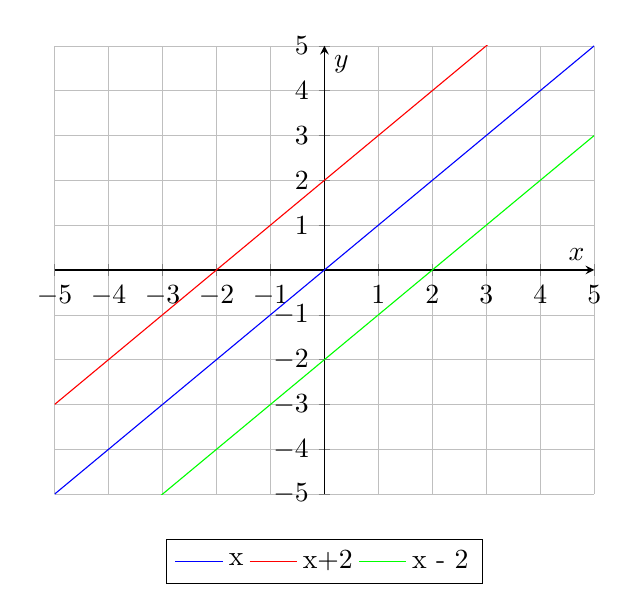
\begin{tikzpicture}%[scale=1.0]
        \begin{axis}[
                xlabel=$x$,
                ylabel=$y$,
                xmax=5,
                xmin=-5,
                ymax=5,
                ymin=-5,
                axis x line=middle,
                axis y line=middle,
                legend style={at={(0.5,-0.1)},
                        anchor=north,legend columns=-1},
                grid=major,
                grid style={line width=.1pt, draw=gray!10},
                major grid style={line width=.2pt,draw=gray!50},
                xtick={-5,-4,-3,-2,-1,0,1,2,3,4,5},
                ytick={-5,-4,-3,-2,-1,0,1,2,3,4,5}
            ]
            \addplot [blue] {x};
            \addlegendentry {x};
            \addplot [red] {x+2};
            \addlegendentry {x+2};
            \addplot [green] {x-2};
            \addlegendentry {x - 2};
        \end{axis}
    \end{tikzpicture}\\~\\
    Wenn wir die Steigungt m in $f(x) = mx + n$ veraendern, passiert Folgendes:
    \begin{itemize}
        \item Gilt $m > 0$, steigt die Gerade.
        \item Gilt $m < 0$ , faellt die Gerade.
    \end{itemize}
    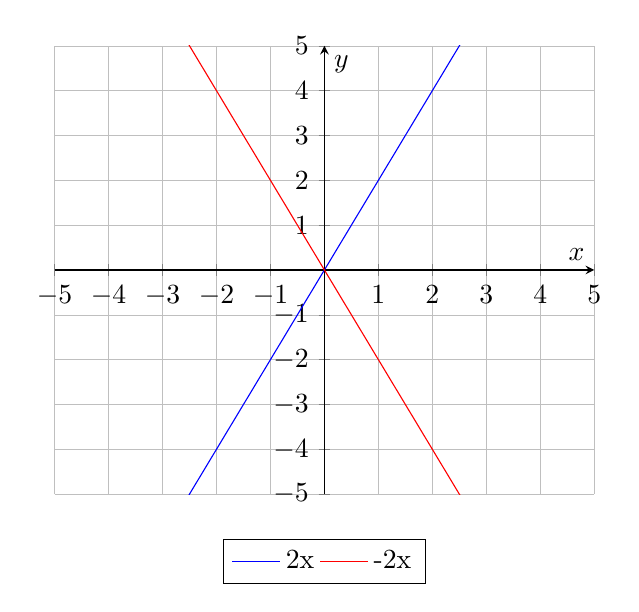
\begin{tikzpicture}%[scale=1.0]
        \begin{axis}[
                xlabel=$x$,
                ylabel=$y$,
                xmax=5,
                xmin=-5,
                ymax=5,
                ymin=-5,
                axis x line=middle,
                axis y line=middle,
                legend style={at={(0.5,-0.1)},
                        anchor=north,legend columns=-1},
                grid=major,
                grid style={line width=.1pt, draw=gray!10},
                major grid style={line width=.2pt,draw=gray!50},
                xtick={-5,-4,-3,-2,-1,0,1,2,3,4,5},
                ytick={-5,-4,-3,-2,-1,0,1,2,3,4,5}
            ]
            \addplot [blue] {x*2};
            \addlegendentry {2x};
            \addplot [red] {x*-2};
            \addlegendentry {-2x};
        \end{axis}
    \end{tikzpicture}

    \subsubsection{Nullstelle berechnen}
    \vspace{-4mm}

    Berechne die Nullstelle der linearen Funktion  $y = 3x + 3$. \\
    Wir setzen die Funktion gleich Null, d.h. wir setzen fuer den y Wert 0 ein: ${\color{red}{0}} = 3x + 3$ \\
    Jetzt muessen wir die Gleichung nach x aufloesen, um die gesuchte Nullstelle zu finden.
    \subsubsection{Steigung berechnen}
    Wir lesen zwei beliebige Punkte ab:
    \[P_0({\color{blue}0}|{\color{red}1}) \text{ und } P_1({\color{blue}4}|{\color{red}3})\]
    und setzen sie in die Steigungsformel ein:
    \begin{align*} m &= \frac{y_1 - y_0}{x_1 - x_0} \\[5px] &= \frac{{\color{red}3} - ({\color{red}1})}{{\color{blue}4} - {\color{blue}0}}\\[5px] &= \frac{2}{4} \\[5px] &= \frac{1}{2} \end{align*}
    \subsubsection{Schnittpunkt berechnen}
    \vspace{-4mm}

    Ein Schnittpunkt existiert nur, wenn die beiden gegebenen Geraden eine unterschiedliche Steigung besitzen.
    \[g\colon~y = {\color{red}2}x + 1\]
    \[h\colon~y = {\color{red}2}x + 3\]
    Die Geraden besitzen dieselbe Steigung das heisst: \textbf{Es existiert kein Schnittpunkt}.\\
    Ansonsten gilt:
    \begin{enumerate}
        \item Funktionsgleichungen gleichsetzen
        \item Gleichung nach x aufloesen
        \item x in eine der beiden Funktionsgleichungen einsetzen, um y zu berechnen
        \item Ergebnis aufschreiben
    \end{enumerate}

    \subsubsection{Umkehrfunktion bilden}
    \vspace{-4mm}

    \begin{enumerate}
        \item Funktionsgleichung nach x aufloesen
        \item x und y vertauschen
    \end{enumerate}

    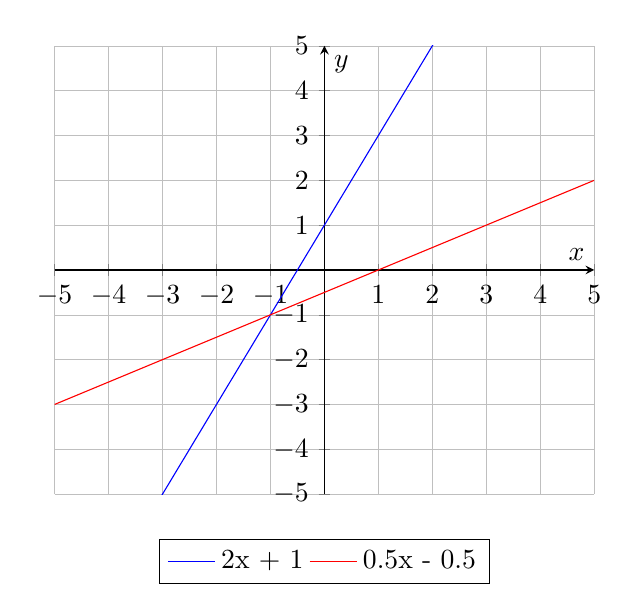
\begin{tikzpicture}%[scale=1.0]
        \begin{axis}[
                xlabel=$x$,
                ylabel=$y$,
                xmax=5,
                xmin=-5,
                ymax=5,
                ymin=-5,
                axis x line=middle,
                axis y line=middle,
                legend style={at={(0.5,-0.1)},
                        anchor=north,legend columns=-1},
                grid=major,
                grid style={line width=.1pt, draw=gray!10},
                major grid style={line width=.2pt,draw=gray!50},
                xtick={-5,-4,-3,-2,-1,0,1,2,3,4,5},
                ytick={-5,-4,-3,-2,-1,0,1,2,3,4,5}
            ]
            \addplot [blue] {x*2+1};
            \addlegendentry {2x + 1};
            \addplot [red] {x*0.5-0.5};
            \addlegendentry {0.5x - 0.5};
        \end{axis}
    \end{tikzpicture}

    \subsection{Quadratische Funktionen}
    \vspace{-4mm}
    \subsubsection{Definition}
    \vspace{-4mm}
    Eine Funktion $f$ mit der Funktionsgleichung $f(x) = ax^2 + bx + c$ heisst quadratische Funktion.
    Der Graph einer quadratischen Funktion ist eine Parabel.

    \subsubsection{Quadratische Funktion Zeichnen}
    \vspace{-4mm}
    Dazu berechnen wir zunaechst einige Funktionswerte:
    \[f(-2) = (-2)^2 = 4\]
    \[f(-1) = (-1)^2 = 1\]
    \[f(0) = 0^2 = 0\]
    \[f(1) = 1^2 = 1\]
    \[f(2) = 2^2 = 4\]
    Der uebersichtlichkeit halber fassen unsere Berechnungen in einer Wertetabelle zusammen:
    \[ \begin{array}{r|c|c|c|c|c} x\text{-Werte} & -2 & -1 & 0 & 1 & 2 \\ \hline y\text{-Werte} & 4 & 1 & 0 & 1 & 4 \\ \end{array}\]
    Wenn wir jetzt die berechneten Punkte in ein Koordinatensystem eintragen und anschliessend die Punkte verbinden, erhalten wir den Graphen der Funktion $f(x)=x^2$ , die sog. Normalparabel.
    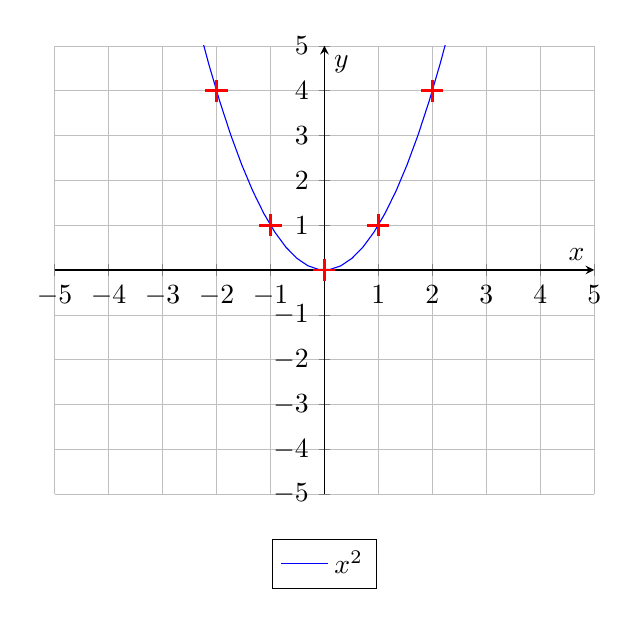
\begin{tikzpicture}%[scale=1.0]
        \begin{axis}[
                xlabel=$x$,
                ylabel=$y$,
                xmax=5,
                xmin=-5,
                ymax=5,
                ymin=-5,
                axis x line=middle,
                axis y line=middle,
                legend style={at={(0.5,-0.1)},
                        anchor=north,legend columns=-1},
                grid=major,
                grid style={line width=.1pt, draw=gray!10},
                major grid style={line width=.2pt,draw=gray!50},
                xtick={-5,-4,-3,-2,-1,0,1,2,3,4,5},
                ytick={-5,-4,-3,-2,-1,0,1,2,3,4,5},
                samples=50
            ]
            \addplot [blue] {x^2};
            \addlegendentry {$x^2$};
            \addplot+[
                mark=+,
                only marks,
                mark size=4pt,
                mark options={line width=1pt},
                mark color=red
            ]
            coordinates
                {(-2,4) (-1,1) (0,0) (1,1) (2,4)};

        \end{axis}
    \end{tikzpicture}

    \subsubsection{Normalparabel nach oben/unten verschieben}
    \vspace{-4mm}
    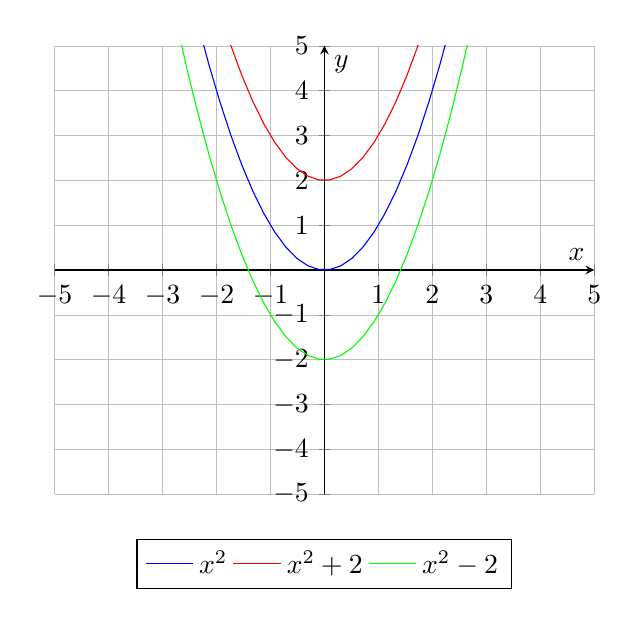
\begin{tikzpicture}%[scale=1.0]
        \begin{axis}[
                xlabel=$x$,
                ylabel=$y$,
                xmax=5,
                xmin=-5,
                ymax=5,
                ymin=-5,
                axis x line=middle,
                axis y line=middle,
                legend style={at={(0.5,-0.1)},
                        anchor=north,legend columns=-1},
                grid=major,
                grid style={line width=.1pt, draw=gray!10},
                major grid style={line width=.2pt,draw=gray!50},
                xtick={-5,-4,-3,-2,-1,0,1,2,3,4,5},
                ytick={-5,-4,-3,-2,-1,0,1,2,3,4,5},
                samples=50
            ]
            \addplot [blue] {x^2};
            \addlegendentry {$x^2$};
            \addplot [red] {x^2+2};
            \addlegendentry {$x^2+2$};
            \addplot [green] {x^2-2};
            \addlegendentry {$x^2-2$};
        \end{axis}
    \end{tikzpicture}
    \begin{equation*} {\color{red}f(x)} + c = \begin{cases} \text{ Verschiebung nach oben} &\text{fuer } c > 0 \\[5px] \text{ Verschiebung nach unten} &\text{fuer } c < 0 \end{cases} \end{equation*}


    \subsubsection{Normalparabel stauchen/strecken}
    \vspace{-4mm}
    Moechte man die Normalparabel stauchen oder strecken, muss man sich die Parabelgleichung $f(x) = ax^2$ anschauen.

    \begin{tabularx}{0.5\textwidth} {
            | >{\raggedright\arraybackslash}c
            | >{\raggedright\arraybackslash}X |}
        \hline
        $a > 1$      & Die Parabel ist nach oben geoeffnet und
        schmaler* als die Normalparabel                         \\ \hline
        $a = 1$      & Die nach oben geoeffnete Normalparabel   \\ \hline
        $0 < a < 1$  & Die Parabel ist nach oben geoeffnet und
        breiter**  als die Normalparabel                        \\ \hline
        $-1 < a < 0$ & Die Parabel ist nach unten geoeffnet und
        breiter**  als die Normalparabel                        \\ \hline
        $a = -1$     & Die nach unten geoeffnete Normalparabel  \\ \hline
        $a < -1$     & Die Parabel ist nach unten geoeffnet und
        schmaler*   als die Normalparabel                       \\ \hline
    \end{tabularx}
    \\~\\
    * gestreckt, ** gestaucht \\~\\
    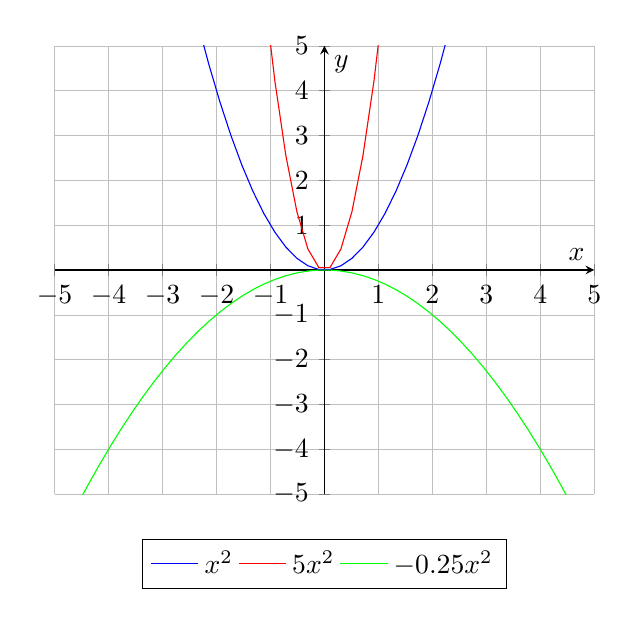
\begin{tikzpicture}%[scale=1.0]
        \begin{axis}[
                xlabel=$x$,
                ylabel=$y$,
                xmax=5,
                xmin=-5,
                ymax=5,
                ymin=-5,
                axis x line=middle,
                axis y line=middle,
                legend style={at={(0.5,-0.1)},
                        anchor=north,legend columns=-1},
                grid=major,
                grid style={line width=.1pt, draw=gray!10},
                major grid style={line width=.2pt,draw=gray!50},
                xtick={-5,-4,-3,-2,-1,0,1,2,3,4,5},
                ytick={-5,-4,-3,-2,-1,0,1,2,3,4,5},
                samples=50
            ]
            \addplot [blue] {x^2};
            \addlegendentry {$x^2$};
            \addplot [red] {5*x^2};
            \addlegendentry {$5x^2$};
            \addplot [green] {-0.25*x^2};
            \addlegendentry {$-0.25x^2$};

        \end{axis}
    \end{tikzpicture}
    \subsubsection{Parabel verschieben entlang der x-Achse}
    \vspace{-4mm}
    \begin{equation*} f({\color{red}x} + d) = \begin{cases} \text{ Verschiebung nach rechts} &\text{fuer } d < 0 \\[5px] \text{ Verschiebung nach links} &\text{fuer } d > 0 \end{cases} \end{equation*}
    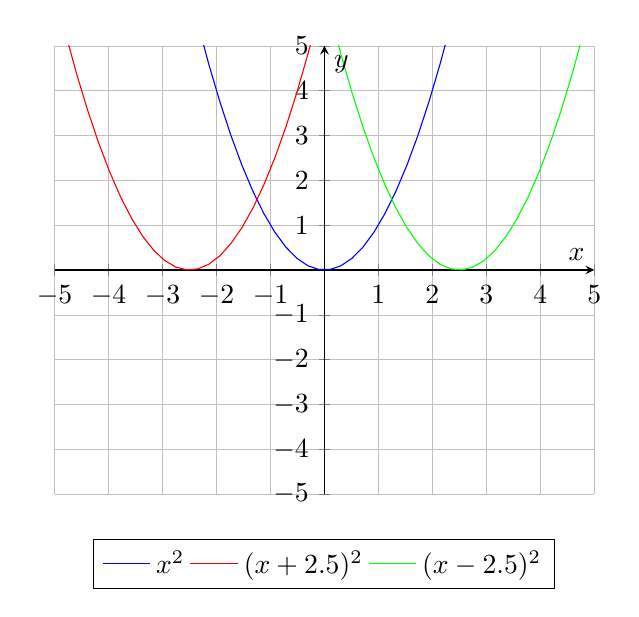
\begin{tikzpicture}%[scale=1.0]
        \begin{axis}[
                xlabel=$x$,
                ylabel=$y$,
                xmax=5,
                xmin=-5,
                ymax=5,
                ymin=-5,
                axis x line=middle,
                axis y line=middle,
                legend style={at={(0.5,-0.1)},
                        anchor=north,legend columns=-1},
                grid=major,
                grid style={line width=.1pt, draw=gray!10},
                major grid style={line width=.2pt,draw=gray!50},
                xtick={-5,-4,-3,-2,-1,0,1,2,3,4,5},
                ytick={-5,-4,-3,-2,-1,0,1,2,3,4,5},
                samples=50
            ]
            \addplot [blue] {x^2};
            \addlegendentry {$x^2$};
            \addplot [red] {(x+2.5)^2};
            \addlegendentry {$(x+2.5)^2$};
            \addplot [green] {(x-2.5)^2};
            \addlegendentry {$(x-2.5)^2$};

        \end{axis}
    \end{tikzpicture}

    \subsubsection{y-Achsenabschnitt berechnen}
    \vspace{-4mm}
    Die x-Koordinate des Schnittpunktes mit der y-Achse ist immer Null. \\
    Bei quadratischen Funktionen laesst sich der y-Achsenabschnitt aus der Funktionsgleichung ablesen: Der y-Achsenabschnitt von $y = ax^2 + bx + {\color{red}c}$ ist $y = {\color{red}c}$.
    \subsubsection{Nullstellen berechnen}
    \begin{enumerate}
        \item Funktionsgleichung gleich Null setzen
        \item Gleichung loesen
    \end{enumerate}
    Da die y-Koordinate eines Schnittpunktes mit der x-Achse immer Null ist, lautet der Ansatz zur Berechnung einer Nullstelle: $y = 0$. Wegen $y = f(x)$ kann man auch $f(x) = 0$ schreiben. \\~\\
    \textbf{Fall 1: $f(x) = ax^2$} \\~\\
    Funktionen vom Typ $f(x) = ax^2$ besitzen als einzige Nullstelle die Null. \\~\\
    \textbf{Fall 2: $f(x) = ax^2 + c$} . \\~\\
    \begin{enumerate}
        \item     Funktionsgleichung gleich Null setzen
        \item     Gleichung nach $x^2$ aufloesen
        \item     Wurzel ziehen
    \end{enumerate}

    \textbf{Fall 3: $f(x) = ax^2 + bx$} . \\~\\
    \begin{enumerate}
        \item     Funktionsgleichung gleich Null setzen
        \item     Gleichung nach $x$ ausklammern
        \item     Faktoren gleich Null setzen
    \end{enumerate}

    \textbf{Fall 4: $f(x) = ax^2 + bx + c$} . \\~\\
    Quadratische Gleichungen dieses Typs loesen wir mit der Mitternachtsformel


    \subsection{Potenzfunktionen}
    \vspace{-4mm}
    \subsubsection{Definition}
    \vspace{-4mm}
    Eine Funktion $f$ mit der Funktionsgleichung $f(x) = x^n \quad \text{ mit } n \in \mathbb{Z}\setminus\{0\}$ heisst Potenzfunktion. \\~\\
    \subsubsection{Gerade Exponenten}
    \vspace{-4mm}
    Als Beispiele dienen die Funktionen $f(x) = x^2$ und $f(x) = x^4$. \\
    Um die Graphen besser zu zeichnen, berechnen wir zunaechst einige Funktionswerte:
    \[\begin{array}{r|c|c|c|c|c|c|c} x & -1{,}5 & {\color{blue}-1} & -0{,}5 & {\color{blue}0} & 0{,}5 & {\color{blue}1} & 1{,}5 \\ \hline x^2 & 2{,}25 & {\color{blue}1} & 0{,}25 & {\color{blue}0} & 0{,}25 & {\color{blue}1} & 2{,}25 \\ \hline x^4 & 5{,}0625 & {\color{blue}1} & 0{,}0625 & {\color{blue}0} & 0{,}0625 & {\color{blue}1} & 5{,}0625 \end{array}\]
    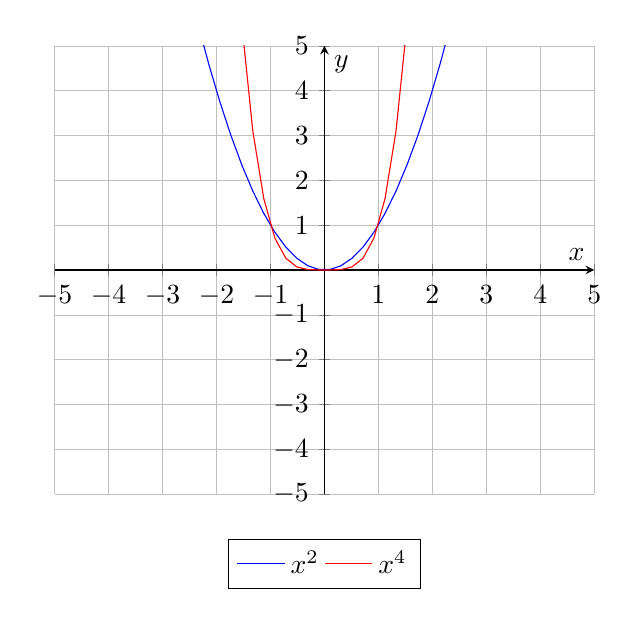
\begin{tikzpicture}%[scale=1.0]
        \begin{axis}[
                xlabel=$x$,
                ylabel=$y$,
                xmax=5,
                xmin=-5,
                ymax=5,
                ymin=-5,
                axis x line=middle,
                axis y line=middle,
                legend style={at={(0.5,-0.1)},
                        anchor=north,legend columns=-1},
                grid=major,
                grid style={line width=.1pt, draw=gray!10},
                major grid style={line width=.2pt,draw=gray!50},
                xtick={-5,-4,-3,-2,-1,0,1,2,3,4,5},
                ytick={-5,-4,-3,-2,-1,0,1,2,3,4,5},
                samples=50
            ]
            \addplot [blue] {x^2};
            \addlegendentry {$x^2$};
            \addplot [red] {x^4};
            \addlegendentry {$x^4$};


        \end{axis}
    \end{tikzpicture}
    \subsubsection{Ungerade Exponenten}
    \vspace{-4mm}
    Als Beispiele dienen die Funktionen $f(x) = x^3$ und $f(x) = x^5$. \\
    Um die Graphen besser zu zeichnen, berechnen wir zunaechst einige Funktionswerte:  \

    \[\begin{array}{r|c|c|c|c|c|c|c} x & -1{,}5 & {\color{blue}-1} & -0{,}5 & {\color{blue}0} & 0{,}5 & {\color{blue}1} & 1{,}5 \\ \hline x^3 & -3{,}375 & {\color{blue}-1} & -0{,}125 & {\color{blue}0} & 0{,}125 & {\color{blue}1} & 3{,}375 \\ \hline x^5 & -7{,}59375 & {\color{blue}-1} & 0{,}03125 & {\color{blue}0} & 0{,}03125 & {\color{blue}1} & 7{,}59375 \end{array}\]
    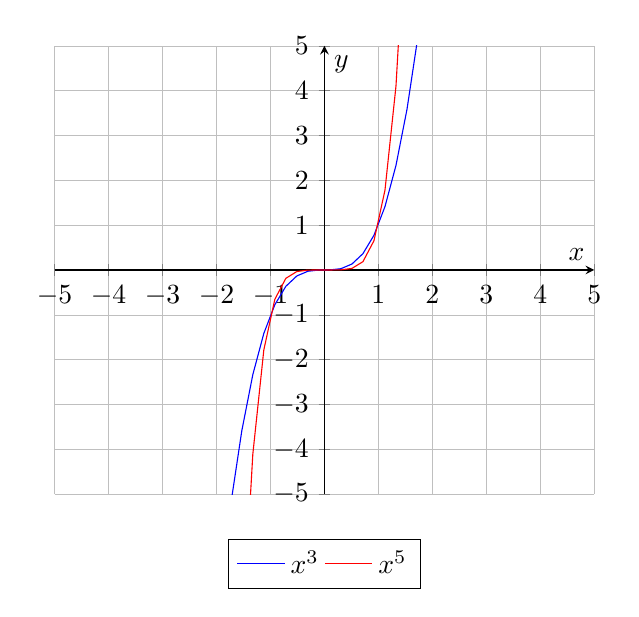
\begin{tikzpicture}%[scale=1.0]
        \begin{axis}[
                xlabel=$x$,
                ylabel=$y$,
                xmax=5,
                xmin=-5,
                ymax=5,
                ymin=-5,
                restrict y to domain=-10:10,
                axis x line=middle,
                axis y line=middle,
                legend style={at={(0.5,-0.1)},
                        anchor=north,legend columns=-1},
                grid=major,
                grid style={line width=.1pt, draw=gray!10},
                major grid style={line width=.2pt,draw=gray!50},
                xtick={-5,-4,-3,-2,-1,0,1,2,3,4,5},
                ytick={-5,-4,-3,-2,-1,0,1,2,3,4,5},
                samples=50
            ]
            \addplot [blue] {x^3};
            \addlegendentry {$x^3$};
            \addplot [red] {x^5};
            \addlegendentry {$x^5$};
        \end{axis}
    \end{tikzpicture}

    \subsubsection{Zusammenfassung der wichtigsten Eigenschaften}
    \vspace{-4mm}
    Potenzfunktionen mit positiven ganzzahligen Exponenten $\boldsymbol{f(x) = x^n}$ haben folgende Eigenschaften:
    \begin{tabular}{l|l|l}
                          & \textbf{n gerade}                 & \textbf{n ungerade}       \\ \hline
        Definitionsmenge  & $\mathbb{D} = \mathbb{R}$         & $\mathbb{D} = \mathbb{R}$ \\ \hline
        Wertemenge        & $\mathbb{W} = \mathbb{R}^{+}_{0}$ & $\mathbb{W} = \mathbb{R}$ \\ \hline
        Symmetrie         & achsensymmetrisch                 & punktsymetrisch           \\
                          & zur y-ache                        & zum K-Ursprung            \\ \hline
        Gemeinsame Punkte & $(-1,1)$,$(0|0)$,$(1|1)$          & $(-1,-1)$,$(0|0)$,$(1|1)$ \\ \hline
    \end{tabular}
    \subsection{Potenzfunktionen mit negativen Exponenten}
    \vspace{-4mm}
    Die Graphen von Potenzfunktionen heissen Hyperbeln n-ter Ordnung, wenn der Exponent negativ ist.
    \subsubsection{Gerade Exponenten}
    \vspace{-4mm}
    Als Beispiele dienen die Funktionen $f(x) = x^{-2}$ und $f(x) = x^{-4}$. \\
    Um die Graphen besser zu zeichnen, berechnen wir zunaechst einige Funktionswerte: \\~\\
    $\begin{array}{r|c|c|c|c|c|c} x & -1{,}5 & {\color{blue}-1} & -0{,}5 & 0{,}5 & {\color{blue}1} & 1{,}5 \\ \hline x^{-2} & 0{,}\bar{4} & {\color{blue}1} & 4 & 4 & {\color{blue}1} & 0{,}\bar{4} \\ \hline x^{-4} & \approx 0{,}1975 & {\color{blue}1} & 16 & 16 & {\color{blue}1} & \approx 0{,}1975 \end{array}$ \\~\\
    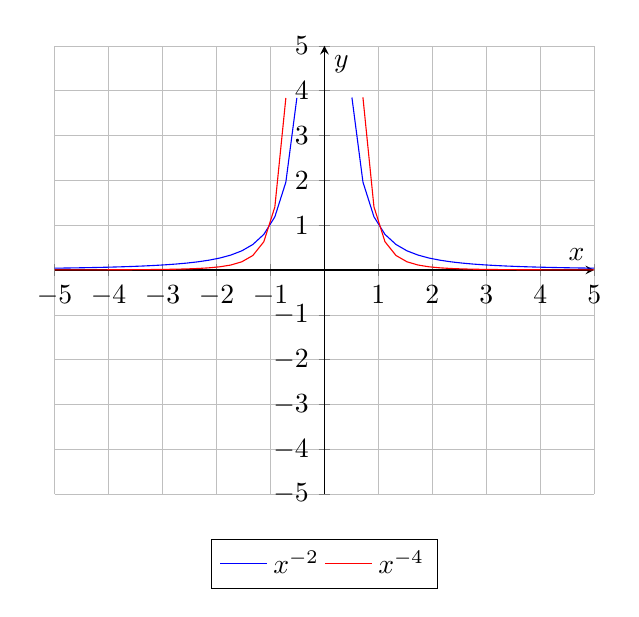
\begin{tikzpicture}%[scale=1.0]
        \begin{axis}[
                xlabel=$x$,
                ylabel=$y$,
                xmax=5,
                xmin=-5,
                ymax=5,
                ymin=-5,
                restrict y to domain=-10:10,
                axis x line=middle,
                axis y line=middle,
                legend style={at={(0.5,-0.1)},
                        anchor=north,legend columns=-1},
                grid=major,
                grid style={line width=.1pt, draw=gray!10},
                major grid style={line width=.2pt,draw=gray!50},
                xtick={-5,-4,-3,-2,-1,0,1,2,3,4,5},
                ytick={-5,-4,-3,-2,-1,0,1,2,3,4,5},
                samples=50
            ]
            \addplot [blue] {x^-2};
            \addlegendentry {$x^{-2}$};
            \addplot [red] {x^-4};
            \addlegendentry {$x^{-4}$};
        \end{axis}
    \end{tikzpicture}
    \subsubsection{Gerade Exponenten}
    \vspace{-4mm}
    Als Beispiele dienen die Funktionen $f(x) = x^{-3}$ und $f(x) = x^{-5}$. \\
    Um die Graphen besser zu zeichnen, berechnen wir zunaechst einige Funktionswerte: \\~\\
    $\begin{array}{r|c|c|c|c|c|c} x & -1{,}5 & {\color{blue}-1} & -0{,}5 & 0{,}5 & {\color{blue}1} & 1{,}5 \\ \hline x^{-3} & \approx -0{,}2963 & {\color{blue}-1} & -8 & 8 & {\color{blue}1} & \approx 0{,}2963 \\ \hline x^{-5} & \approx -0{,}1317 & {\color{blue}-1} & -32 & 32 & {\color{blue}1} & \approx 0{,}1317 \end{array}$ \\~\\
    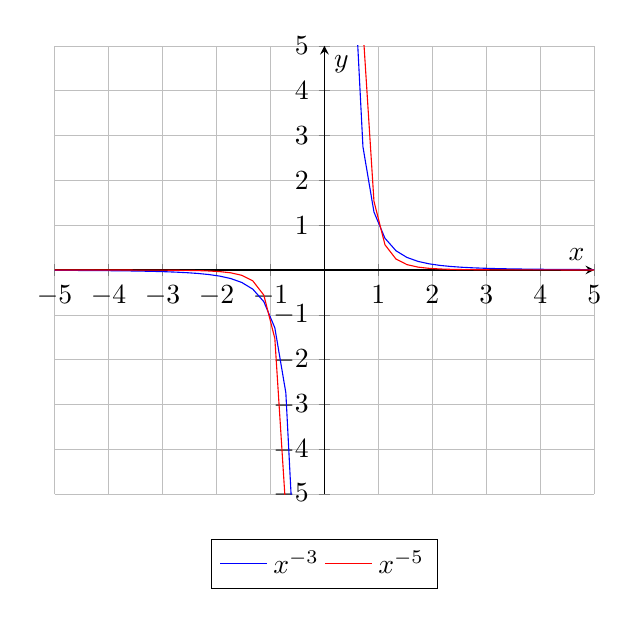
\begin{tikzpicture}%[scale=1.0]
        \begin{axis}[
                xlabel=$x$,
                ylabel=$y$,
                xmax=5,
                xmin=-5,
                ymax=5,
                ymin=-5,
                restrict y to domain=-10:10,
                axis x line=middle,
                axis y line=middle,
                legend style={at={(0.5,-0.1)},
                        anchor=north,legend columns=-1},
                grid=major,
                grid style={line width=.1pt, draw=gray!10},
                major grid style={line width=.2pt,draw=gray!50},
                xtick={-5,-4,-3,-2,-1,0,1,2,3,4,5},
                ytick={-5,-4,-3,-2,-1,0,1,2,3,4,5},
                samples=50
            ]
            \addplot [blue] {x^-3};
            \addlegendentry {$x^{-3}$};
            \addplot [red] {x^-5};
            \addlegendentry {$x^{-5}$};
        \end{axis}
    \end{tikzpicture}

    \subsubsection{Zusammenfassung der wichtigsten Eigenschaften}
    \vspace{-4mm}
    Potenzfunktionen mit negativen ganzzahligen Exponenten $\boldsymbol{f(x) = x^{-n}}$ haben folgende Eigenschaften:
    \begin{tabular}{l|l|l}
                          & \textbf{n gerade}                       & \textbf{n ungerade}                     \\ \hline
        Definitionsmenge  & $\mathbb{D} = \mathbb{R}\setminus\{0\}$ & $\mathbb{D} = \mathbb{R}\setminus\{0\}$ \\ \hline
        Wertemenge        & $\mathbb{W} = \mathbb{R}^{+}$           & $\mathbb{W} = \mathbb{R}\setminus\{0\}$ \\ \hline
        Symmetrie         & achsensymmetrisch                       & punktsymetrisch                         \\
                          & zur y-ache                              & zum K-Ursprung                          \\ \hline
        Gemeinsame Punkte & $(-1,1)$,$(1|1)$                        & $(-1,-1)$,$(1|1)$                       \\ \hline
        Asymptoten        & x-Achse, y-Achse                        & x-Achse, y-Achse                        \\ \hline
    \end{tabular}


    \subsection{Wurzelfunktion}
    \vspace{-4mm}
    \subsubsection{Definition}
    \vspace{-4mm}
    Wurzelfunktionen sind die Umkehrfunktionen von Potenzfunktionen.
    Die Eigenschaften der Funktionen unterscheiden sich danach, ob die (Wurzel-)Exponenten gerade oder ungerade sind.
    \subsubsection{Gerader Wurzelexponent}
    \vspace{-4mm}
    Wir wollen die Umkehrfunktion der Potenzfunktion $y = x^2$ bilden.\\
    Eine Umkehrfunktion existiert immer dann, wenn die Funktion entweder streng monoton steigend oder streng monoton fallend ist.
    Bei der Funktion $y = x^2$ treten jedoch beide Faelle auf. Daraus folgt: Die Funktion  $y = x^2$
    ist fuer $x \in \mathbb{R}$ nicht umkehrbar.\\~\\
    \textbf{Loesung}\\~\\
    Wir beschraenken die Definitionsmenge auf einen Bereich, in dem die Funktion entweder nur streng monoton fallend ($x \leq 0$) oder nur streng monoton steigend ($x \geq 0$) verlaeuft.\\~\\
    \textbf{Fall 1:} $x \leq 0$\\~\\
    Fuer $x \leq 0$ ist die Funktion $y = x^2$ streng monoton fallend und somit umkehrbar:
    \begin{align*} & &&{\color{orange}\text{1) Funktionsgleichung nach $x$ aufloesen}} \\[5px] f\colon\; y &= x^2 &&{\color{darkgray}| \text{ Wurzel ziehen}} \\[5px] \sqrt{y} &= \sqrt{x^2} \\[5px] \sqrt{y} &= |x| &&{\color{darkgray}| \text{ Betrag aufloesen: } |x| = -x \text{ wegen } x \leq 0} \\[5px] \sqrt{y} &= -x &&{\color{darkgray}|\, \cdot (-1)} \\[5px] -\sqrt{y} &= x &&{\color{darkgray}| \text{ Seiten vertauschen}} \\[5px] x &= -\sqrt{y} \\[5px] & &&{\color{orange}\text{2) $x$ und $y$ vertauschen}} \\[5px] f^{-1}\colon\; y &= -\sqrt{x} \end{align*}
    Um die Graphen der Funktionen ordentlich zu zeichnen, fertigen wir zwei Wertetabellen an.
    \[ \phantom{^{-1}}f\colon\; \begin{array}{r|c|c|c|c|c} x & -2 & -1{,}5 & -1 & -0{,}5 & 0 \\ \hline y & 4 & 2{,}25 & 1 & 0{,}25 & 0 \end{array}\]
    Die Wertetabelle von $f^{-1}$ erhaelt man durch Vertauschen der Zeilen der Wertetabelle von $f$.
    \[f^{-1}\colon\; \begin{array}{r|c|c|c|c|c} x & 4 & 2{,}25 & 1 & 0{,}25 & 0 \\ \hline y & -2 & -1{,}5 & -1 & -0{,}5 & 0 \end{array}\]
    \begin{center}
        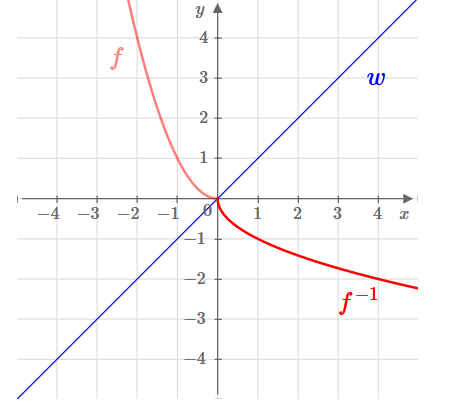
\includegraphics[scale=0.7]{wurzelfunktion1}
    \end{center}
    \textbf{Fall 2:} $x \geq 0$\\~\\
    Fuer ist die Funktion$x \geq 0$ streng monoton steigend und somit umkehrbar:
    \begin{align*} & &&{\color{orange}\text{1) Funktionsgleichung nach $x$ aufloesen}} \\[5px] f\colon\; y &= x^2 &&{\color{darkgray}| \text{ Wurzel ziehen}} \\[5px] \sqrt{y} &= \sqrt{x^2} \\[5px] \sqrt{y} &= |x| &&{\color{darkgray}| \text{ Betrag aufloesen: } |x| = x \text{ wegen } x \geq 0} \\[5px] \sqrt{y} &= x &&{\color{darkgray}| \text{ Seiten vertauschen}} \\[5px] x &= \sqrt{y} \\[5px] & &&{\color{orange}\text{2) $x$ und $y$ vertauschen}} \\[5px] f^{-1}\colon\; y &= \sqrt{x} \end{align*}
    Um die Graphen der Funktionen ordentlich zu zeichnen, fertigen wir zwei Wertetabellen an.
    \[\phantom{^{-1}}f\colon\; \begin{array}{r|c|c|c|c|c} x & 0 & 0{,}5 & 1 & 1{,}5 & 2 \\ \hline y & 0 & 0{,}25 & 1 & 2{,}25 & 4 \end{array}\]
    Die Wertetabelle von $f^{-1}$ erhaelt man durch Vertauschen der Zeilen der Wertetabelle von $f$.
    \[f^{-1}\colon\; \begin{array}{r|c|c|c|c|c} x & 0 & 0{,}25 & 1 & 2{,}25 & 4 \\ \hline y & 0 & 0{,}5 & 1 & 1{,}5 & 2 \end{array}\]

    \begin{center}
        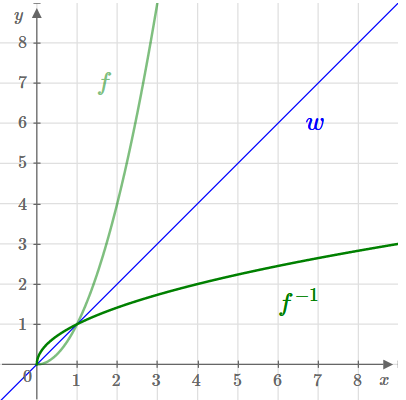
\includegraphics[scale=0.7]{wurzelfunktion2}
    \end{center}
    \subsubsection{Ungerader Wurzelexponent}
    \vspace{-4mm}
    Wir wollen die Umkehrfunktion der Potenzfunktion $y = x^3$ bilden. \\
    Da Potenzfunktionen mit ungeraden Exponenten in $\mathbb{R}$ ganz streng monoton steigend sind, muessen wir die Definitionsmenge nicht einschraenken, um eine Umkehrfunktion zu bilden.
    \begin{align*} & &&{\color{orange}\text{1) Funktionsgleichung nach $x$ aufloesen}} \\[5px] f\colon\; y &= x^3 &&{\color{darkgray}| \text{ Wurzel ziehen}} \\[5px] \sqrt[3]{y} &= \sqrt[3]{x^3} \\[5px] \sqrt[3]{y} &= x &&{\color{darkgray}| \text{ Seiten vertauschen}} \\[5px] x &= \sqrt[3]{y} \\[5px] & &&{\color{orange}\text{2) $x$ und $y$ vertauschen}} \\[5px] f^{-1}\colon\; y &= \sqrt[3]{x} \end{align*}
    Um die Graphen der Funktionen ordentlich zu zeichnen, fertigen wir zwei Wertetabelle an.
    \[\phantom{^{-1}}f\colon\; \begin{array}{r|c|c|c|c|c|c|c|c|c} x & -2 & -1{,}5 & -1 & -0{,}5 & 0 & 0{,}5 & 1 & 1{,}5 & 2 \\ \hline y & -8 & -3{,}375 & -1 & -0{,}125 & 0 & 0{,}125 & 1 & 3{,}375 & 8 \end{array}\]
    Die Wertetabelle von $f^{-1}$ erhaelt man durch Vertauschen der Zeilen der Wertetabelle von $f$.
    \[f^{-1}\colon\; \begin{array}{r|c|c|c|c|c|c|c|c|c} x & -8 & -3{,}375 & -1 & -0{,}125 & 0 & 0{,}125 & 1 & 3{,}375 & 8 \\ \hline x & -2 & -1{,}5 & -1 & -0{,}5 & 0 & 0{,}5 & 1 & 1{,}5 & 2 \end{array}\]
    \begin{center}
        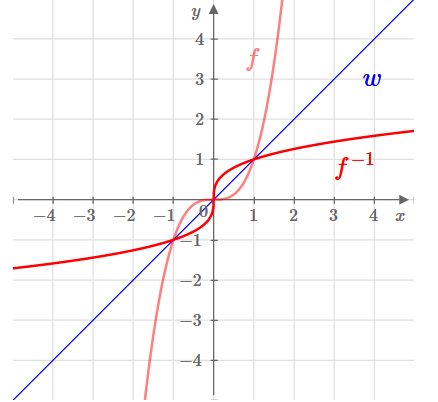
\includegraphics[scale=0.7]{wurzelfunktion3}
    \end{center}

\end{multicols}